% ----------------------------------------------------------
% Capítulo 4 - Resultados e discussão
% ----------------------------------------------------------
\chapter{Resultados e discussão}
\label{cap_resultados}

Nos seis voos de teste, a memória por quadrantes e a amostragem por intervalo enviaram o mesmo número de recortes por voo. A primeira escolhe oportunidades de observação conforme cada ponto do terreno atravessa a imagem. A segunda distribui os envios regularmente ao longo do vídeo. A comparação considera quantos recipientes cada método localizou no mapa, quantos alertas ficaram sem correspondência e quanto tempo o detector levou para reconhecer cada recipiente na imagem. A inferência integral fornece a referência a 40~m. A telemetria de 26 voos e os ensaios de bancada na Jetson permitem estimar o custo energético de levar o detector a bordo.

\section{Desempenho do detector nos recortes de validação}
\label{sec_res_detector}

Mesmo quando o recorte contém um recipiente, o YOLO11n pode deixar de reconhecê-lo. Na validação, a mAP$_{50}$ das doze classes estabilizou-se perto de 0,30 enquanto a perda de treino ainda diminuía. A época~17 obteve a melhor mAP$_{50\text{--}95}$ e forneceu os pesos usados nas comparações de seleção. O treino terminou na época~27 por parada antecipada (Figura~\ref{fig_treino_curvas}).

\begin{figure}[!htbp]
  \centering
  \caption{Evolução do treinamento do YOLO11n na base MBG-V2}
  \label{fig_treino_curvas}
  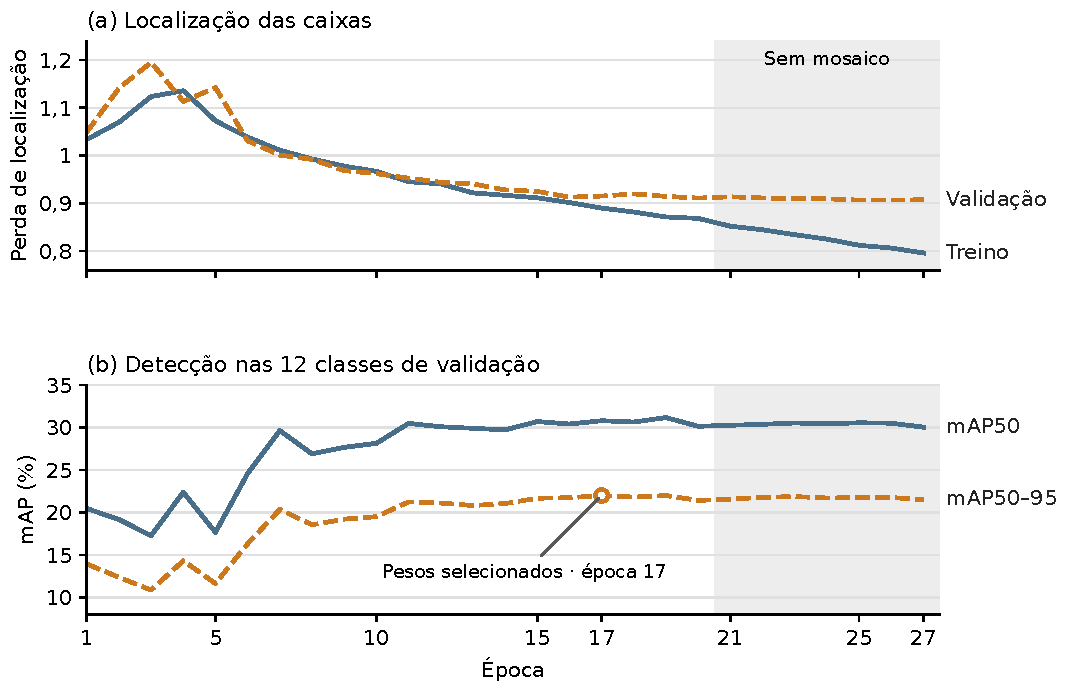
\includegraphics[width=\textwidth]{figuras/fig_treino_curvas.pdf}
  \fonte{Elaborado pelo autor com os registros das 27 épocas. Em (a), valores menores indicam melhor localização das caixas. Em (b), valores maiores indicam melhor detecção nas regiões de validação F e I. As métricas abrangem as doze classes. O círculo marca o maior mAP$_{50\text{--}95}$, na época 17. A faixa cinza corresponde às épocas 21 a 27, realizadas sem mosaico de imagens.}
\end{figure}

Caixas d'água e bueiros tiveram as maiores AP$_{50}$ entre as seis classes principais (Tabela~\ref{tab_detector}). O detector encontrou a maioria das piscinas anotadas, mas também classificou muitas regiões dos recortes como piscina sem que a caixa prevista correspondesse à anotação. As seis classes raras alcançaram AP$_{50}$ de no máximo 0,18. Pela Equação~\eqref{eq_spx}, o mesmo recipiente ocupa menos pixels à medida que o $GSD$ aumenta. Estimar a altura máxima de inspeção pela Equação~\eqref{eq_hmax} exigiria medir o recall em função desse tamanho.

\begin{table}[!htbp]
  \centering
  \caption{Desempenho do YOLO11n por classe na validação (regiões F e I)}
  \label{tab_detector}
  \begin{tabular}{lcccccc}
    \hline
    Classe & Caixas & $P$ & $R$ & AP$_{50}$ & AP$_{50\text{-}95}$ & F1 máximo \\
    \hline
    Caixa d'água & 4.272 & 0,81 & 0,91 & 0,93 & 0,80 & 0,89 \\
    Vaso de planta & 1.239 & 0,37 & 0,30 & 0,20 & 0,10 & 0,35 \\
    Bueiro & 975 & 0,81 & 0,87 & 0,89 & 0,56 & 0,86 \\
    Piscina & 664 & 0,56 & 0,87 & 0,77 & 0,60 & 0,77 \\
    Pneu & 888 & 0,47 & 0,44 & 0,38 & 0,23 & 0,47 \\
    Balde & 624 & 0,43 & 0,24 & 0,25 & 0,16 & 0,36 \\
    \hline
    Média das seis classes & -- & 0,57 & 0,60 & 0,57 & 0,41 & 0,61 \\
    \hline
  \end{tabular}
  \fonte{Elaborado pelo autor com o avaliador da Ultralytics 8.4.183. Em 7.944 recortes, $P$ e $R$ usam o limiar que maximiza a curva suavizada de F1 médio entre classes. O F1 máximo usa o melhor limiar de cada classe. A AP integra por trapézios a curva de precisão interpolada em 101 níveis de recall. A validação conserva 10\% dos recortes vazios, o que reduz as oportunidades de falso positivo em relação à varredura do quadro completo.}
\end{table}

\subsection{Detecção de pneus em comparação com Souza (2025)}

Na quinta divisão da MBG-V2, que contém os mesmos quatro voos usados aqui para validação, o maior F1 para pneus tabulado por \citeonline[Tabelas 3.1 e A.7]{souza2025aedes} foi de 0,59. A autora avaliou o YOLOv8s em diferentes faixas de confiança e variou a fração de um pneu que precisava permanecer no recorte para conservar a anotação. O YOLO11n deste trabalho alcançou F1 máximo de 0,47 para pneus. Além do tratamento dos recortes, os treinos diferem em escopo. Souza usou 22 voos para treinar um detector de pneus, enquanto o YOLO11n aprendeu a distinguir doze classes em 14 voos.

\section{Detecção nos seis voos de teste}
\label{sec_qualidade_teste}

\subsection{Recipientes localizados e falsos alarmes}
\label{sec_resultados_quadrantes}

Nos seis voos a 40~m, havia 1.924 recipientes anotados nas seis classes avaliadas. A memória por quadrantes solicitou 8.796 recortes, em média 5,59~recortes/s, e localizou 1.079 desses recipientes. O intervalo, ajustado para enviar tantos recortes quanto a memória em cada voo (Seção~\ref{sec_metodo_quadrantes}), localizou 1.054. Com a memória, o recall geográfico foi 1,30~ponto percentual maior e houve 435 falsos alarmes a menos no mapa (Tabela~\ref{tab_resultados_quadrantes}).

A diferença se concentrou nos voos 16 e 23, em cada um dos quais a memória localizou 11 recipientes a mais que o intervalo. Nos demais, a diferença variou de zero a dois. Já a redução dos falsos alarmes ocorreu nos seis voos (Figura~\ref{fig_resultados_quadrantes}a, b).

\begin{table}[!htbp]
  \centering
  \caption{Localização no mapa e primeiro alerta visual nos seis voos originais a 40~m}
  \label{tab_resultados_quadrantes}
  \small
  \setlength{\tabcolsep}{5pt}
  \begin{tabular}{@{}lrrr@{}}
    \hline
    Medida & Quadrantes & Intervalo pareado & Integral \\
    \hline
    Recortes processados & 8.796 & 8.796 & 1.131.600 \\
    Referências localizadas no mapa & 1.079 & 1.054 & 1.400 \\
    Recall geográfico (\%) & 56,08 & 54,78 & 72,77 \\
    Falsos alarmes no mapa & 1.291 & 1.726 & 5.892 \\
    Precisão dos alertas no mapa (\%) & 45,53 & 37,91 & 19,20 \\
    \hline
    Trilhas confirmadas na imagem & 1.160 & 1.137 & 1.448 \\
    Trilhas com alerta em até 1~s (\%) & 21,6 & 11,9 & 63,0 \\
    Mediana do primeiro alerta (s) & 1,37 & 2,40 & 0,07 \\
    Percentil 90 do primeiro alerta (s) & 4,31 & 4,75 & 1,31 \\
    \hline
  \end{tabular}
  \fonte{Elaborado pelo autor. Cada recipiente conta uma vez por voo. A precisão no mapa é a fração dos focos previstos que correspondem a um recipiente anotado da mesma classe a até 1,0~m. Os demais focos previstos contam como falsos alarmes. A fração com alerta em até 1~s considera os 1.924 recipientes. A mediana e o percentil 90 consideram as trilhas que cada método confirmou na imagem.}
\end{table}

Pela contagem das células de 0,5~m cujo centro apareceu em pelo menos um recorte, o intervalo mostrou ao detector 98,17\% do terreno filmado e a memória, 94,49\%. Embora tenha coberto mais terreno, o intervalo localizou menos recipientes. No cálculo da área, basta que uma célula apareça uma vez, por mais breve que seja a vista. Já a localização exige que ao menos uma vista permita reconhecer o recipiente e que a posição estimada fique a até 1,0~m da referência no mapa.

A inferência integral examinou os 24 recortes de todos os quadros. Com cerca de 129 vezes o número de recortes da memória, localizou mais 321 recipientes e gerou mais 4.601 falsos alarmes. Mesmo examinando o vídeo inteiro, 524 recipientes ficaram sem localização correta no mapa.

\begin{figure}[!htbp]
  \centering
  \caption{Diferenças de localização por voo e tempo até o primeiro alerta a 40~m}
  \label{fig_resultados_quadrantes}
  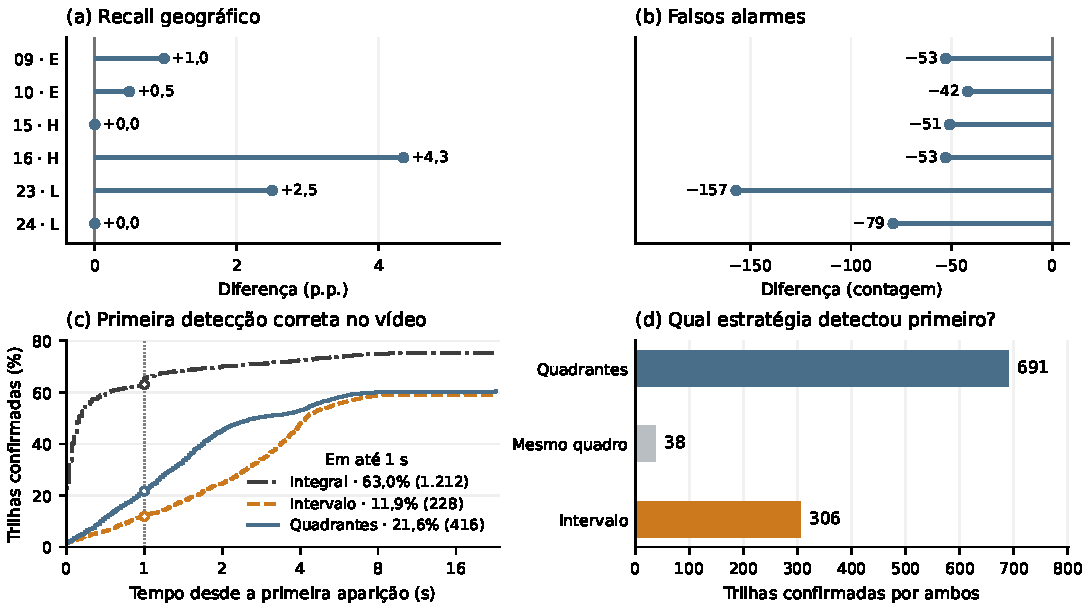
\includegraphics[width=\textwidth]{figuras/fig_resultados_quadrantes.pdf}
  \fonte{Elaborado pelo autor. Em (a) e (b), subtrai-se o resultado do intervalo do obtido pelos quadrantes. Em (c), as curvas mostram, a cada instante, a fração das 1.924 trilhas anotadas que já receberam confirmação visual. Em (d), contam-se apenas as 1.035 trilhas que tanto a memória quanto o intervalo confirmaram.}
\end{figure}

\subsection{Tempo até a primeira detecção correta no vídeo}
\label{sec_primeiro_alerta}

Na imagem, o primeiro alerta corresponde ao primeiro quadro com detecção da classe anotada, confiança de pelo menos 0,5 e IoU de pelo menos 0,5. No primeiro segundo após a aparição anotada, a memória confirmou 416 recipientes e o intervalo, 228 (Figura~\ref{fig_resultados_quadrantes}c). A memória envia poucos recortes por vez em muitos instantes do voo, enquanto o intervalo concentra o mesmo total em quadros mais espaçados. Assim, quando um recipiente aparece logo após um envio por intervalo, a espera até a próxima oportunidade de detectá-lo é maior.

Nas 1.035 trilhas que as duas estratégias confirmaram, a memória antecipou o primeiro alerta em 691 casos (Figura~\ref{fig_resultados_quadrantes}d). Para esse conjunto comum, a espera mediana caiu de 2,37~s com o intervalo para 1,33~s com a memória. Esses tempos seguem o relógio do vídeo. A Seção~\ref{sec_res_jetson_memoria} considera também a fila e a execução no computador de bordo.

Ao ampliar o prazo para cinco segundos, a vantagem dos quadrantes concentrou-se nas 1.685 trilhas com menor variação do movimento da aeronave, com 50 confirmações a mais que o intervalo. Nas 216 trilhas de maior variação, o intervalo confirmou cinco a mais (Figura~\ref{fig_alertas_por_movimento}). Assim, os seis voos não demonstram vantagem dos quadrantes durante as manobras.

\begin{figure}[!htbp]
  \centering
  \caption{Confirmação visual em até cinco segundos segundo a variação do movimento da aeronave}
  \label{fig_alertas_por_movimento}
  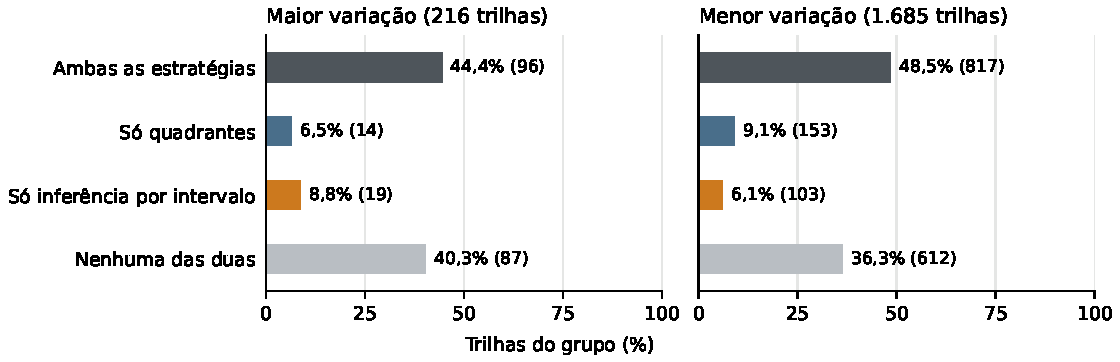
\includegraphics[width=\textwidth]{figuras/fig_alertas_movimento_quadrantes.pdf}
  \fonte{Elaborado pelo autor. No grupo de maior variação, o vetor de velocidade horizontal se afastou mais de 0,5~m/s de sua média na janela. As barras mostram o percentual de cada grupo e os números entre parênteses, a contagem. O recipiente pode sair da imagem antes do quinto segundo. As 23 trilhas sem cinco segundos completos de vídeo e telemetria integram os resultados gerais.}
\end{figure}

\subsection{Efeito da altura simulada na detecção}
\label{sec_resultados_escala}

Ao passar de 40 para 80~m de altura equivalente, o mesmo recipiente ocupa metade da largura e da altura originais na entrada do detector. A Figura~\ref{fig_escala_por_classe} acompanha essa redução junto ao recall de cada classe. Os quadros, os recortes escolhidos e os recipientes de referência permaneceram os mesmos nas cinco escalas (Seção~\ref{sec_metodo_altura_integral}).

\begin{figure}[!htbp]
  \centering
  \caption{Recall geográfico e tamanho aparente dos recipientes por classe e altura equivalente}
  \label{fig_escala_por_classe}
  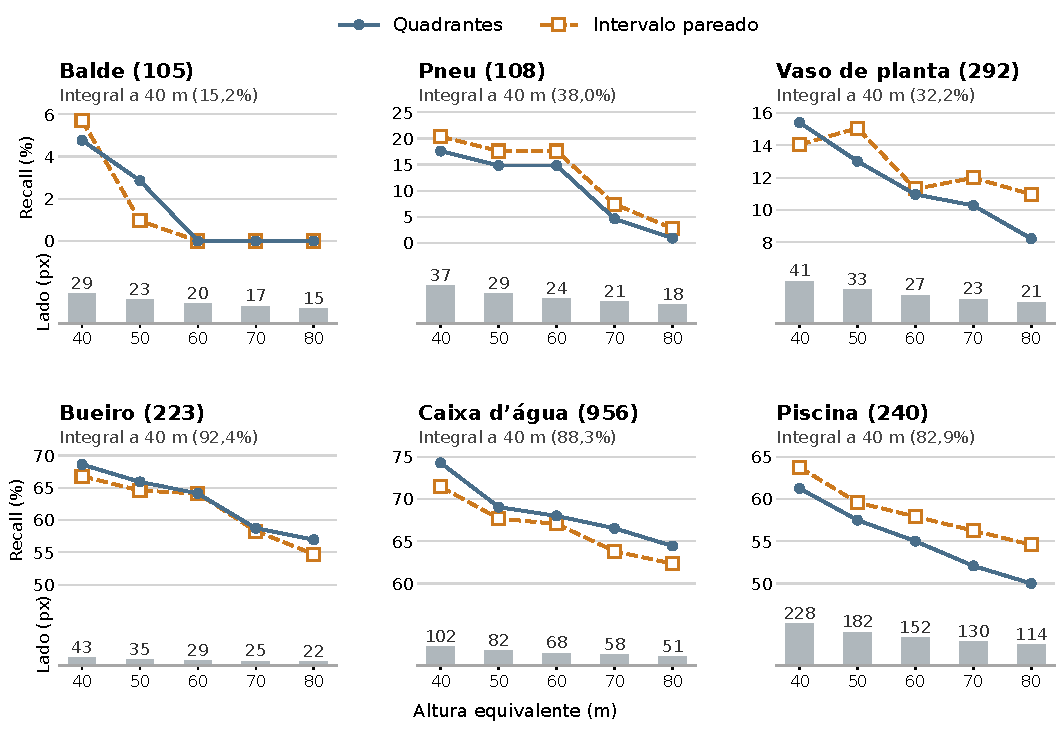
\includegraphics[width=\textwidth]{figuras/fig_escala_classes_quadrantes.pdf}
  \fonte{Elaborado pelo autor. O eixo de recall tem escala própria em cada classe. O cabeçalho indica o total anotado e o recall da integral a 40~m. As barras mostram o lado médio das caixas em pixels e usam a mesma escala nos três painéis de cada linha. Para cada recipiente, usa-se a mediana de $\sqrt{\text{largura}\times\text{altura}}$ de suas caixas anotadas a 40~m e aplica-se o fator $40/h$ à altura $h$.}
\end{figure}

Os baldes, com as menores caixas na imagem, já eram difíceis de localizar na altura original. Mesmo a inferência integral localizou apenas 16 dos 105 baldes a 40~m. A partir de 60~m, nenhum dos dois métodos de seleção localizou um balde. Os pneus também se tornaram raros no mapa. Dos 108 anotados, apenas um foi localizado pelos quadrantes e três pelo intervalo a 80~m.

Entre as caixas d'água localizadas pelos quadrantes a 40~m, as que continuaram localizadas a 80~m já eram maiores na imagem original. O lado mediano era de 113~pixels nesse grupo e de 88~pixels entre as que deixaram de ser localizadas. Entre classes distintas, porém, tamanhos semelhantes nem sempre corresponderam a resultados próximos. A 80~m, bueiros e vasos de planta tinham lados médios de 21,7 e 20,5~pixels, respectivamente, mas os quadrantes localizaram 57,0\% dos bueiros e apenas 8,2\% dos vasos.

Nos seis voos, o recall das duas estratégias caiu para cerca de 46\% a 80~m (Figura~\ref{fig_deteccao_escala}). A vantagem dos quadrantes passou de 25 recipientes a 40~m para quatro a 80~m. A 60~m, o intervalo localizou dois a mais. Os totais próximos encobrem diferenças por classe. A 80~m, os quadrantes localizaram 20 caixas d'água a mais, enquanto o intervalo localizou 11 piscinas a mais.

\begin{figure}[!htbp]
  \centering
  \caption{Efeito da altura equivalente sobre a localização no mapa e o alerta no primeiro segundo}
  \label{fig_deteccao_escala}
  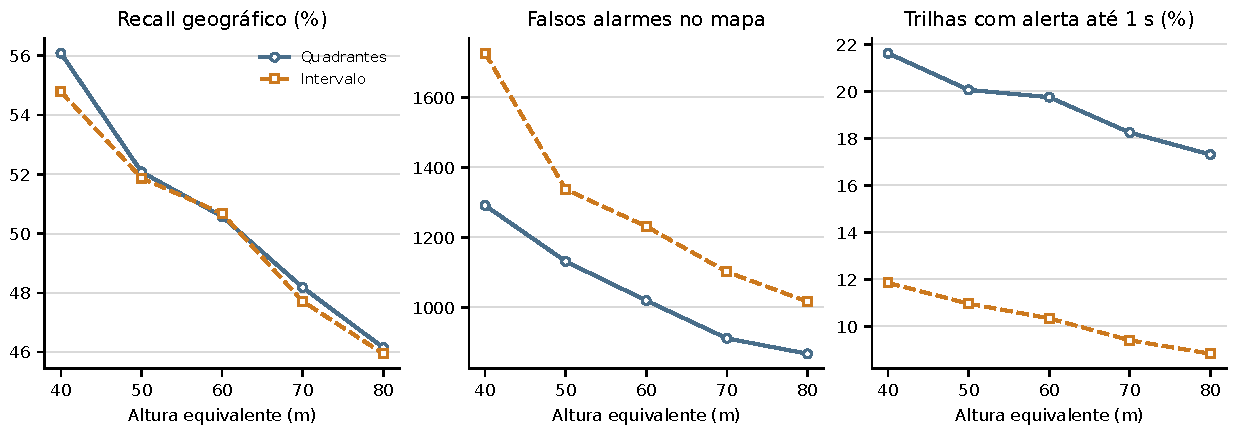
\includegraphics[width=\textwidth]{figuras/fig_escala_quadrantes.pdf}
  \fonte{Elaborado pelo autor. Cada ponto reúne as 1.924 trilhas dos seis voos com 8.796 recortes por estratégia. O recall e os falsos alarmes referem-se ao mapa. A confirmação até o primeiro segundo é medida na imagem desde a primeira aparição de cada recipiente.}
\end{figure}

Em todas as alturas simuladas, os quadrantes produziram menos falsos alarmes no mapa e confirmaram mais recipientes no primeiro segundo. Mesmo a 80~m, confirmaram quase o dobro nesse prazo (333 contra 170). A simulação isola a mudança de escala e de contexto visual nos recortes. Em um voo real a outra altura, também mudariam a faixa de terreno visível e os instantes de passagem pelos quadrantes.

\subsection{Quanto da primeira vista se repete ao cruzar um quadrante?}
\label{sec_sobreposicao_passagens}

Nos seis voos a 40~m, foi possível comparar 4.042 pares de recortes enviados pela memória na entrada de um ponto na imagem e na primeira mudança de quadrante desse ponto. O intervalo mediano entre as duas vistas foi de 3,50~s, e o segundo recorte voltou a cobrir, em média, 83,3\% da área projetada do primeiro. Ao dividir a área comum pela união das áreas dos dois recortes, obtém-se a IoU. Sua média foi de 0,737, e 75,1\% dos pares tiveram IoU acima de 0,75 (Figura~\ref{fig_sobreposicao_distribuicao}).

Nos 953 pares com ao menos um recipiente anotado nas duas vistas, houve 1.401 oportunidades de comparar o reconhecimento de um mesmo recipiente, correspondentes a 1.312 trilhas distintas (Figura~\ref{fig_sobreposicao_distribuicao}a). Em 140 oportunidades, o detector reconheceu o recipiente somente na travessia. Nesses casos, a segunda vista permitiu detectar um recipiente que já estava visível na entrada. O inverso ocorreu quase com a mesma frequência, com 136 reconhecimentos exclusivos da entrada. A grande sobreposição do terreno, portanto, não tornou as duas vistas equivalentes para a detecção.

\begin{figure}[!htbp]
  \centering
  \caption{Reconhecimento do recipiente nas duas vistas e sobreposição dos recortes e das caixas no terreno}
  \label{fig_sobreposicao_distribuicao}
  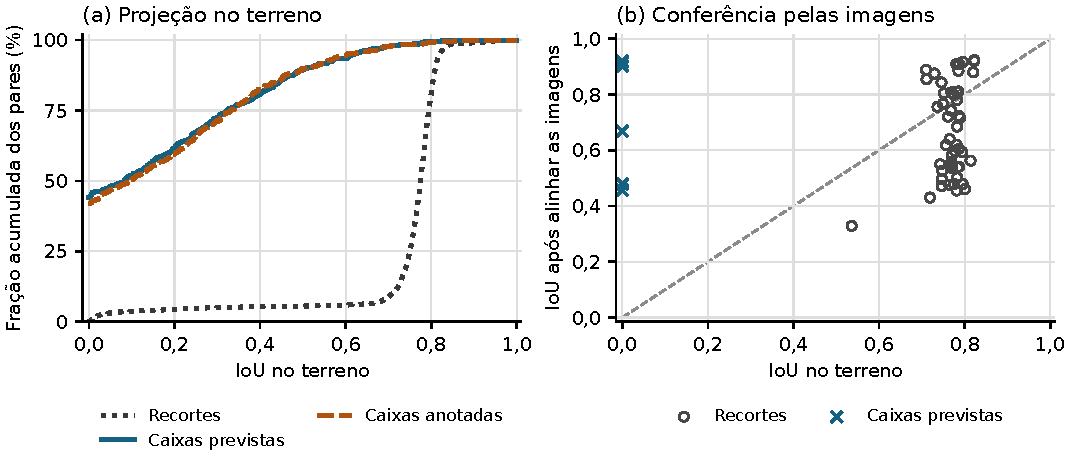
\includegraphics[width=\textwidth]{figuras/fig_sobreposicao_distribuicao.pdf}
  \fonte{Elaborado pelo autor. Em (a), cada uma das 1.401 oportunidades corresponde a um recipiente anotado em um par de recortes de entrada e travessia. Em (b), a primeira coluna distribui os 4.042 pares de recortes pelas faixas de IoU. As outras duas colunas consideram os mesmos 648 casos de reconhecimento nas duas vistas e comparam, respectivamente, as caixas previstas entre si e as anotadas entre si. Cada coluna soma 100\%, salvo arredondamento.}
\end{figure}

Nos 648 casos em que o detector reconheceu o recipiente nas duas vistas, as caixas previstas se sobrepuseram pouco ao serem projetadas no terreno. A distância mediana entre os centros foi de 1,36~m e a IoU média, de 0,180. Em 285 casos (44,0\%), as caixas ficaram sem nenhuma área em comum. A projeção das caixas anotadas nas mesmas imagens produziu resultados próximos, com IoU média de 0,184 e distância mediana de 1,33~m. A diferença de posição entre as vistas, portanto, também aparece quando se usa a marcação manual.

Dos 180 pares de recortes amostrados para verificar a sobreposição diretamente nas imagens, 49 atenderam aos critérios de alinhamento pelos pixels. Em seis desses pares, o detector reconheceu um recipiente nas duas vistas, como no exemplo do bueiro da Figura~\ref{fig_sobreposicao_pares}.

\begin{figure}[!htbp]
  \centering
  \caption{O mesmo recipiente nos recortes de entrada e de travessia em três voos}
  \label{fig_sobreposicao_pares}
  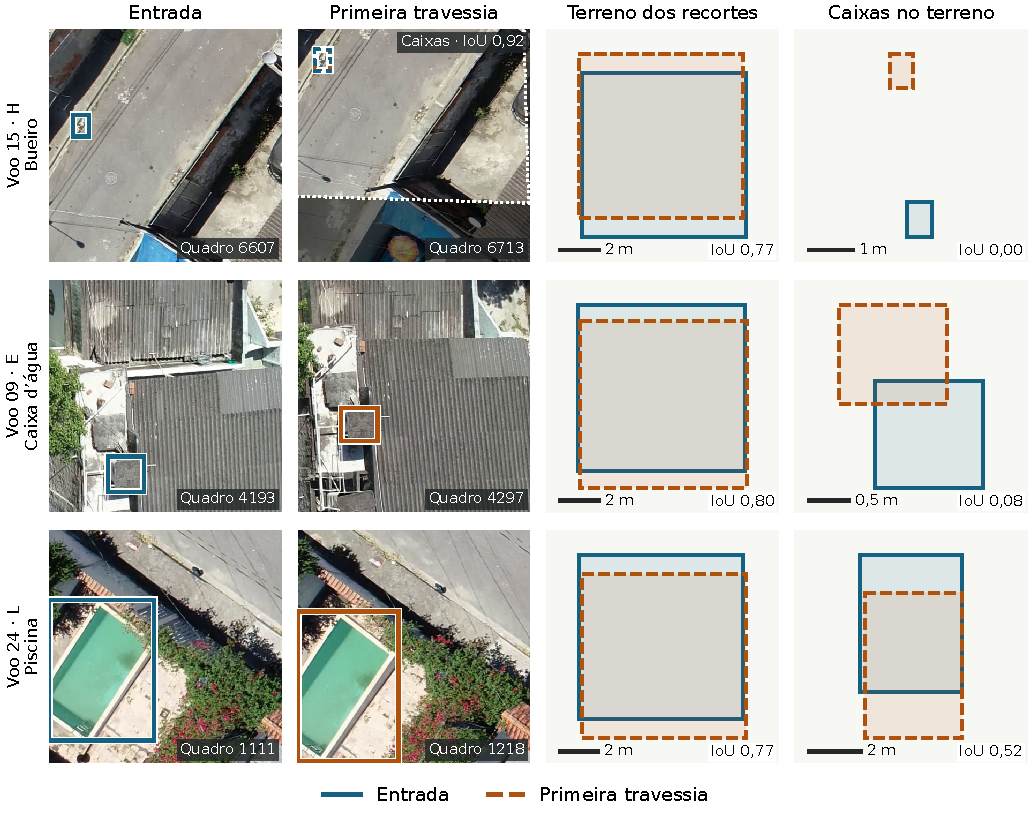
\includegraphics[width=\textwidth]{figuras/fig_sobreposicao_pares.pdf}
  \fonte{Elaborado pelo autor a partir da MBG-V2 \cite{smt2024mbgv2}. Nos dois painéis à direita, cada par está centralizado e orientado pelos lados do recorte de entrada. As barras dão a escala. Na segunda foto do bueiro, a faixa escurecida mostra a área ausente na entrada e o contorno azul tracejado mostra onde a caixa da primeira vista ficou após o alinhamento pelos pixels.}
\end{figure}

A Figura~\ref{fig_sobreposicao_pares} mostra três exemplos próximos aos percentis 10, 50 e 90 da IoU das caixas no terreno. Escolheram-se classes e regiões distintas, com o recipiente inteiro nos dois recortes e a mesma orientação de câmera nas duas vistas. Para o exemplo de IoU zero, exigiu-se também alinhamento visual validado. No voo~15, as duas caixas do bueiro têm IoU de 0,92 depois de alinhar as imagens, mas ficam separadas no mapa. No voo~24, as caixas da piscina ainda se sobrepõem no terreno, com IoU de 0,52. Essa diferença ajuda a interpretar a escolha da distância entre centros para associar os focos (Seção~\ref{sec_metodo_alertas}).

Fixar a origem da malha na primeira posição válida do GPS de cada voo produziu resultado semelhante. Nos 4.051 pares dessa configuração, a IoU média dos recortes foi 0,736. Nos 624 casos em que o detector reconheceu o recipiente nas duas imagens, a IoU média das caixas foi 0,190.

\subsection{Mapa das detecções e das anotações projetadas no terreno}
\label{sec_mapa_final_quadrantes}

A Figura~\ref{fig_mapa_final_quadrantes} compara o mapa que a memória por quadrantes produziu ao fim de cada voo com as posições de referência dos recipientes anotados. A malha de 8,64~m orienta a escolha dos recortes, mas os focos podem ficar entre seus pontos, pois a posição de cada foco vem das caixas detectadas. A referência é a mediana dos centros das caixas anotadas de cada trilha após a projeção no terreno. Como a base não fornece posições medidas em campo e as duas projeções usam o mesmo GSD e a mesma telemetria, a distância entre um foco e sua referência indica a concordância com as anotações projetadas.

Dos 2.370 focos previstos e das 1.924 referências, formaram-se 1.079 pares no raio de avaliação de 1,0~m. Entre esses acertos, a distância mediana foi de 0,33~m e o percentil 90, de 0,81~m.

\begin{figure}[!htbp]
  \centering
  \caption{Mapa final da memória por quadrantes e posições de referência dos recipientes nos seis voos}
  \label{fig_mapa_final_quadrantes}
  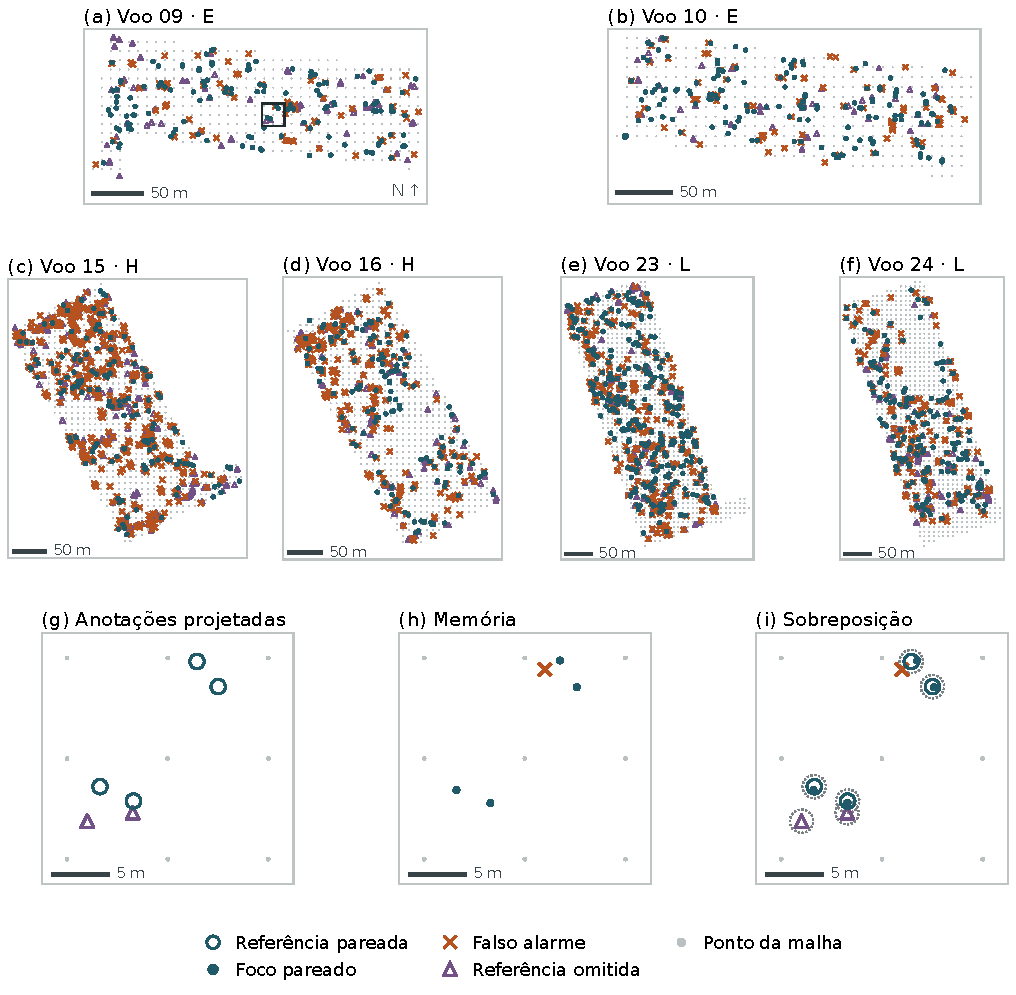
\includegraphics[width=\textwidth]{figuras/fig_mapa_final_quadrantes.pdf}
  \fonte{Elaborado pelo autor a partir das detecções e das trilhas anotadas da MBG-V2 \cite{smt2024mbgv2}. Os pontos cinza mostram a malha que orientou a seleção dos recortes. Os painéis (g) a (i) ampliam o quadrado de 21,6~m de lado marcado no voo~09 e mostram, na mesma escala, a referência, o resultado da memória e a sobreposição. Em (i), os círculos pontilhados indicam o raio de avaliação de 1,0~m.}
\end{figure}

No detalhe do voo~09, havia seis recipientes anotados e cinco focos previstos. Quatro focos encontraram par. O quinto estava a 1,06~m da referência mais próxima da mesma classe, já associada a outro foco a 0,52~m.

\section{Potência e inclinação em cruzeiro: comparação com a telemetria}
\label{sec_curva_potencia_voos}

A curva da Figura~\ref{fig_curva_potencia} prevê menor potência a 8~m/s do que a 4~m/s pela redução da potência induzida. Os dois regimes de cruzeiro da MBG-V2 permitem verificar essa queda. A posição do mínimo e o aumento da potência em velocidades maiores dependem da extrapolação do modelo.

\subsection{Comparação em trechos de cruzeiro}

Para o quadrirrotor de 1,4~kg da Figura~\ref{fig_curva_potencia}, o arrasto $D$ e o peso determinam a tração $T=\sqrt{(mg)^2+D^2}$ e a inclinação $\alpha_d=\arctan[D/(mg)]$. Com a tração dividida entre quatro rotores, calcula-se $v_h$ pela Equação~\eqref{eq_vh} e resolve-se a Equação~\eqref{eq_glauert} para a velocidade induzida positiva. A Equação~\eqref{eq_pv} reúne as parcelas induzida, de perfil e parasita na potência mecânica $P(V;m)$. Como a base não mede o vento, a simulação assume vento nulo e iguala a velocidade horizontal relativa ao ar à registrada em relação ao solo.

Como a curva prevê a potência necessária para manter o voo retilíneo e nivelado, a comparação com a bateria considerou trechos em que a altitude, a velocidade e a direção permaneceram quase constantes. Para uma altitude nominal de 40~m em relação à decolagem, os percentis 5 e 95 da altitude registrada foram de 39,8 e 40,1~m. Adotaram-se como velocidades de referência as medianas observadas nas campanhas, de 4,1~m/s nas regiões B a M e de 7,9~m/s na região A (Tabela~\ref{tab_campanhas}).

A seleção principal reteve 1.103 das 1.303 janelas consecutivas de cinco segundos (84,7\%). Cada janela precisava atender aos seis critérios da Figura~\ref{fig_sensibilidade_cruzeiro}. O limite entre registros restringe a interpolação, e o limite vertical exclui subidas e descidas mesmo quando a altitude ainda está próxima da referência.

O limite do vetor velocidade rejeita curvas mesmo quando o módulo varia pouco. O outro limite horizontal verifica se a média do módulo na janela se aproxima do cruzeiro da campanha. A potência de cada janela é a média temporal do produto da tensão pela corrente. Cada ponto da Figura~\ref{fig_potencia_telemetria} reúne as medianas de velocidade e potência de um voo, dando igual peso a voos de durações diferentes.

Para comparar a previsão mecânica com a potência elétrica da bateria, adotou-se $P_{av}=0$ na Equação~\eqref{eq_pel} e ajustou-se a conversão $\widehat P_{el}=P(V;m_0)/\eta$. A mediana das razões $P(V_i;m_0)/P_{el,i}$ nos 14 voos das regiões de treinamento (Seção~\ref{sec_detector}) deu $\eta=0{,}836$. Esse fator efetivo incorpora aviônicos e simplificações aerodinâmicas e foi mantido nos outros 12 voos.

\begin{figure}[!htbp]
  \centering
  \caption{Potência elétrica prevista pelo modelo ajustado e registrada pela bateria em cruzeiro}
  \label{fig_potencia_telemetria}
  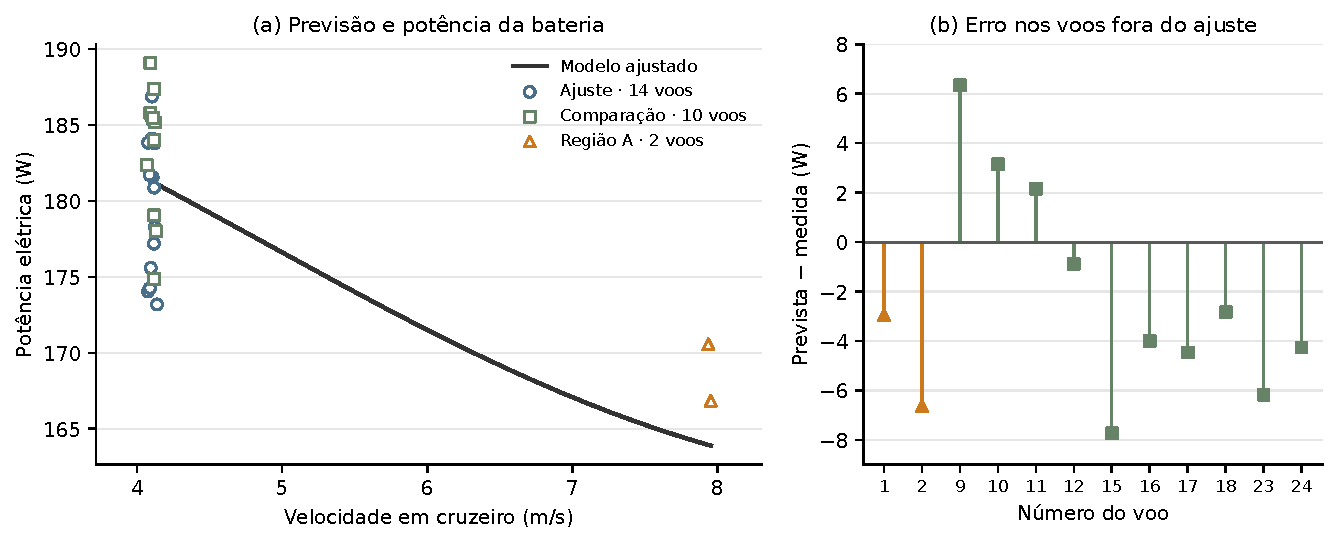
\includegraphics[width=\textwidth]{figuras/fig_potencia_telemetria.pdf}
  \fonte{Elaborado pelo autor a partir do modelo e da telemetria da MBG-V2 \cite{smt2024mbgv2}. Em (a), a linha indica a potência prevista e cada símbolo representa um voo. A ampliação ao centro mostra os 24 voos próximos de 4,1~m/s. Os rótulos identificam os voos 08 (ajuste) e 18 (comparação), cujas medianas quase coincidem. Em (b), valores positivos indicam potência prevista acima da registrada nos voos reservados.}
\end{figure}

Nos dez voos reservados da campanha de 4,1~m/s, o erro absoluto médio foi de 4,2~W. A média dos erros percentuais absolutos por voo foi de 2,3\%. Nos dois voos mais rápidos, o modelo reproduziu a queda de potência entre campanhas, mas subestimou a potência medida em ambos (Figura~\ref{fig_potencia_telemetria}b).

O erro de potência foi mais sensível à tolerância do vetor de velocidade horizontal. Ao reduzir o desvio admissível de 0,5 para 0,3~m/s, a seleção perdeu 9,6~min de cruzeiro e o erro absoluto médio aumentou cerca de 1~W. Variar a tolerância de altitude manteve tanto o tempo selecionado quanto o erro (Figura~\ref{fig_sensibilidade_cruzeiro}).

\begin{figure}[!htbp]
  \centering
  \caption{Efeito dos critérios de cruzeiro sobre o tempo selecionado e o erro de potência}
  \label{fig_sensibilidade_cruzeiro}
  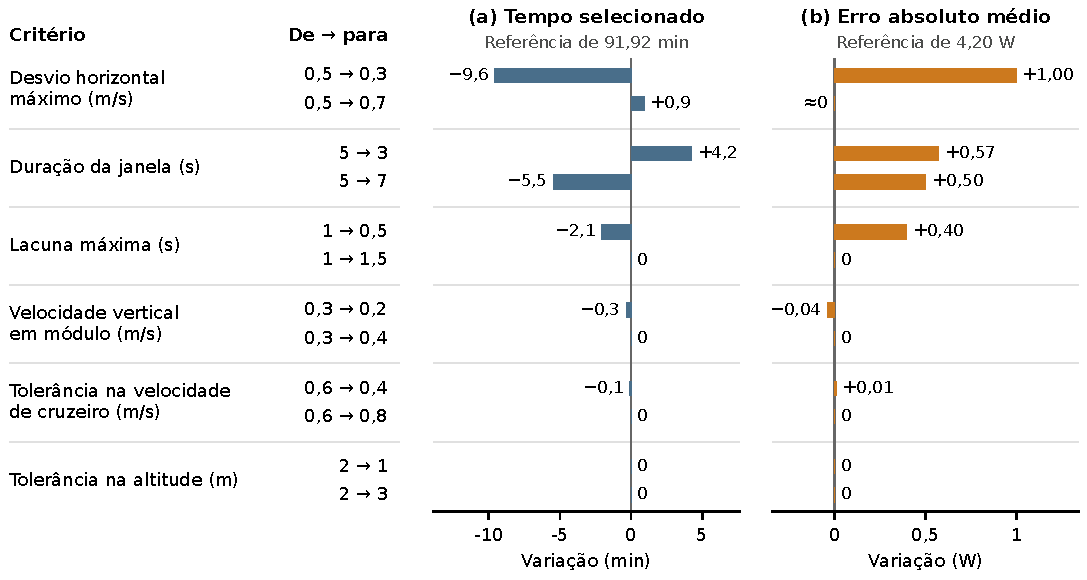
\includegraphics[width=\textwidth]{figuras/fig_sensibilidade_cruzeiro.pdf}
  \fonte{Elaborado pelo autor. Cada linha altera um único critério do valor adotado para a alternativa indicada. Em (a), a variação é relativa aos 91,92~min de cruzeiro nos 26 voos. Em (b), reajusta-se $\eta$ nos mesmos 14 voos e compara-se o erro absoluto médio nos dez voos reservados da campanha de 4,1~m/s com o erro de referência de 4,20~W.}
\end{figure}

\subsection{Inclinação prevista e observada em cruzeiro}

A inclinação oferece uma verificação independente do ajuste à potência. Em cruzeiro nivelado, a tangente do ângulo de inclinação, $\tan\theta$, dá a razão entre a resistência ao avanço e o peso (Equação~\eqref{eq_equilibrio}). Com vento nulo e toda a resistência atribuída ao arrasto parasita, o modelo prevê que $\tan\theta$ cresça com o quadrado da velocidade (Equação~\eqref{eq_fe}).

Os registros de arfagem, rolamento e guinada permitiram estimar a inclinação na direção do deslocamento. Nas passadas a até $15^\circ$ do eixo principal de cada voo, calculou-se a mediana de $\tan\theta$ separadamente na ida e na volta. A média das duas medianas deu o mesmo peso a cada sentido. O voo~12 ficou fora dessa análise por ter registros válidos em um único sentido.

Mesmo com a potência ajustada à telemetria, a aeronave inclinou-se mais do que o modelo previa nas duas campanhas (Figura~\ref{fig_verificacao_telemetria}c). A passagem de 4,1 para 7,9~m/s multiplicou $\tan\theta$ por 1,85. A relação quadrática, com $f_e=0{,}02$~m$^2$, previa um fator de 3,73. Dois regimes, sem medição do vento, são insuficientes para determinar como o arrasto varia com a velocidade. Por isso, o custo de transportar o kit é estimado com a curva ajustada à potência da bateria, na faixa de velocidades observada (Seção~\ref{sec_balanco_por_voo}).

\section{Área imageada e duração das aparições}
\label{sec_res_telemetria}

O $GSD$ de cada voo foi estimado a partir do movimento da aeronave e do deslocamento dos recipientes na imagem (Seção~\ref{sec_base_condicoes}). A Equação~\eqref{eq_pegada} dá a largura $w$ da faixa usada no cálculo da energia por área e o comprimento $L$ que determina o tempo de visibilidade. Na Figura~\ref{fig_verificacao_telemetria}, $P_{el}$ e $V$ são as medianas de potência e velocidade de cada voo.

\subsection{Energia por área}

Em cruzeiro retilíneo, a Equação~\eqref{eq_e_area} prevê um gasto específico $e=P_{el}/(Vw)$. A Figura~\ref{fig_verificacao_telemetria}a mostra a diferença percentual em relação à previsão de cruzeiro, calculada como $100(e_{\mathrm{voo}}/e-1)$, em que $e_{\mathrm{voo}}$ é a energia fornecida pela bateria por unidade de área imageada (Equação~\eqref{eq_e_voo}). Nos 24 voos das regiões B a M, o gasto por área ficou, na mediana, 5\% acima do previsto. A razão entre o gasto observado e o previsto pode ser escrita como
\begin{equation*}
  \frac{e_{\mathrm{voo}}}{e} =
  \underbrace{\frac{\bar{P}_{el}}{P_{el}}}_{\text{potência}}\;
  \underbrace{\frac{V}{\bar{V}}}_{\text{velocidade}}\;
  \underbrace{\frac{s\,w}{A_{\mathrm{img}}}}_{\text{revisitas}},
\end{equation*}
em que $\bar{P}_{el}=E/t_{\mathrm{voo}}$ e $\bar{V}=s/t_{\mathrm{voo}}$ são as médias de potência e de velocidade no trecho de duração $t_{\mathrm{voo}}$ e distância $s$. Os dois primeiros fatores expressam quanto os valores usados na previsão diferem dessas médias. O terceiro compara a faixa que seria varrida em linha reta, $sw$, à área efetivamente imageada, $A_{\mathrm{img}}$, que conta o terreno revisitado uma única vez.

\begin{figure}[H]
  \centering
  \caption{Energia por área, tempo de visibilidade e inclinação nos voos da MBG-V2}
  \label{fig_verificacao_telemetria}
  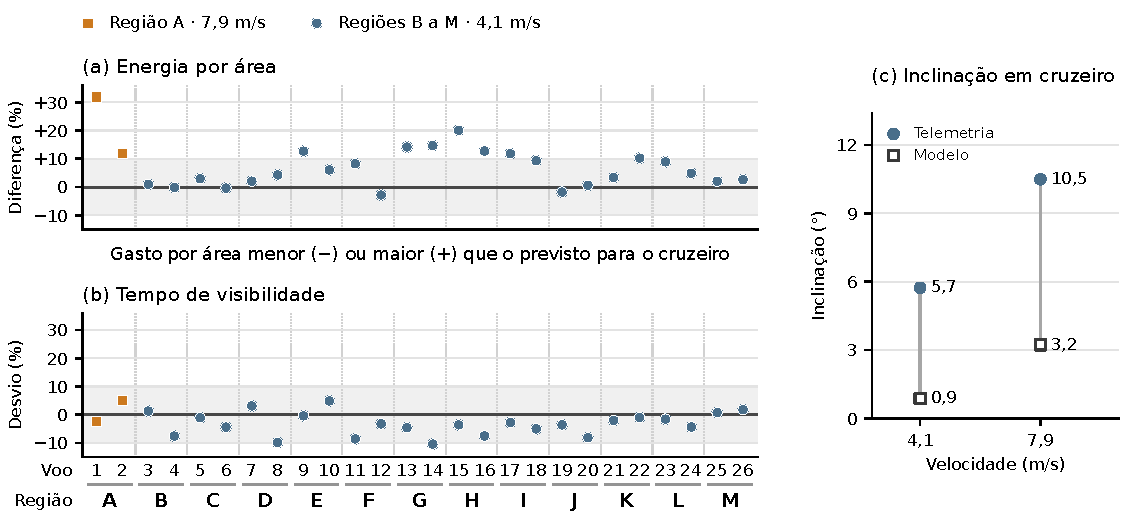
\includegraphics[width=\textwidth]{figuras/fig_telemetria_fisica.pdf}
  \fonte{Elaborado pelo autor a partir da MBG-V2 \cite{smt2024mbgv2}. Em (a) e (b), cada ponto representa um voo e cada letra, uma região. A linha de zero indica concordância com a previsão de cruzeiro (Equações~\eqref{eq_e_area} e~\eqref{eq_visibilidade}) e a faixa cinza cobre desvios de até 10\% em ambos os sentidos. Em (c), os círculos mostram a inclinação obtida da mediana das tangentes de 23 voos a 4,1~m/s e de dois a 7,9~m/s. Os quadrados mostram a previsão para a velocidade mediana de cada grupo.}
\end{figure}

Nos 23 voos de B a M com distância e energia disponíveis para o mesmo intervalo, os fatores de potência e velocidade ficaram entre 0,94 e 1,03. Quanto maior a sobreposição, maior o gasto por área em relação à previsão retilínea. A correlação de 0,98 entre o fator de revisitas e a razão entre medida e previsão descreve como o gasto estimado se distribui entre os fatores, pois as duas grandezas usam a mesma área reconstruída e o fator de revisitas faz parte da própria razão. A exclusão do voo~14 se restringe a essa decomposição. Seu balanço de energia considera o intervalo comum (Seção~\ref{sec_base_integridade}).

Na região A, a energia por área supera a previsão em 32\% no voo~01 e em 12\% no voo~02. Nesses dois voos a 7,9~m/s, acelerações e curvas ocupam uma fração maior do trecho. A velocidade usada na estimativa ficou 27\% acima da média do trajeto no voo~01 e 7\% acima no voo~02. O fator de revisitas é de apenas 1,03.

\subsection{Tempo de visibilidade}

O tempo $t_v=L/V$ da Equação~\eqref{eq_visibilidade} prevê por quanto tempo um alvo permanece visível ao atravessar toda a faixa. Nos 26 voos, o desvio entre a duração mediana das trilhas e a previsão variou de $-10\%$ a $+5\%$, com mediana de $-3\%$ (Figura~\ref{fig_verificacao_telemetria}b). As trilhas do próprio voo também serviram para ajustar o $GSD$ usado no cálculo de $L$. A comparação verifica a consistência desse ajuste com as durações observadas. Uma curva ou o fim do vídeo pode interromper a observação antes de o recipiente atravessar toda a faixa.

A Figura~\ref{fig_visibilidade_por_classe} mostra a distribuição das durações nas 12 classes anotadas. Cada trilha recebeu a previsão $L/V$ do seu voo. Como essa previsão é comum a todas as classes de um voo, sua distribuição por classe depende de quais voos contêm os recipientes. As caixas d'água, presentes nos 26 voos, ficaram visíveis por uma mediana de 3,38~s na região A e de 7,07~s nas regiões B a M.

\begin{figure}[H]
  \centering
  \caption{Tempo de visibilidade previsto e duração das trilhas anotadas por classe e campanha}
  \label{fig_visibilidade_por_classe}
  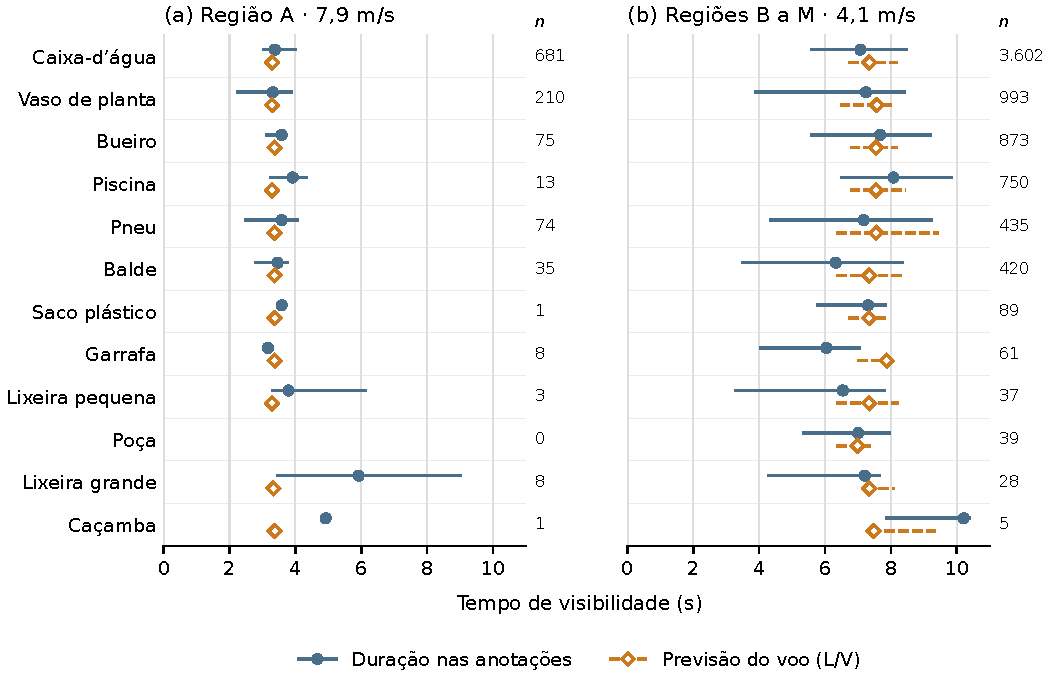
\includegraphics[width=\textwidth]{figuras/fig_visibilidade_por_classe.pdf}
  \fonte{Elaborado pelo autor a partir das 8.441 trilhas da MBG-V2 \cite{smt2024mbgv2}. A duração anotada vai do primeiro ao último quadro com o recipiente na imagem, incluindo ambos, à taxa de quadros do vídeo. Os símbolos indicam a mediana e os segmentos vão do percentil 10 ao 90. Cada trilha conta uma vez. A coluna $n$ informa quantas trilhas há em cada grupo.}
\end{figure}

Nas regiões B a M, baldes e piscinas tiveram previsões medianas semelhantes. O percentil 10 da duração anotada foi de 3,50~s para os baldes e de 6,51~s para as piscinas. As aparições mais curtas exigem envios mais frequentes ao detector, pois o recipiente pode entrar e sair da imagem entre dois envios.

\section{Desempenho e consumo do computador de bordo}
\label{sec_res_jetson}

\subsection{Vazão, energia e qualidade por configuração}
\label{sec_bancada_motores}

Na Jetson Orin Nano em modo de 25~W, transferir a inferência em FP32 da CPU para a GPU pelo provedor CUDA do ONNX Runtime elevou a vazão de 7,3 para 43,2 imagens/s e reduziu em cerca de 74\% a energia total por imagem (Figura~\ref{fig_bancada_vazao_energia}). A redução da energia por imagem também ocorreu no PyTorch com TorchScript ao passar de FP32 para FP16, embora nesse caso a vazão tenha diminuído.

\begin{figure}[!htbp]
  \centering
  \caption{Vazão e energia por inferência do YOLO11n em nove configurações da Jetson}
  \label{fig_bancada_vazao_energia}
  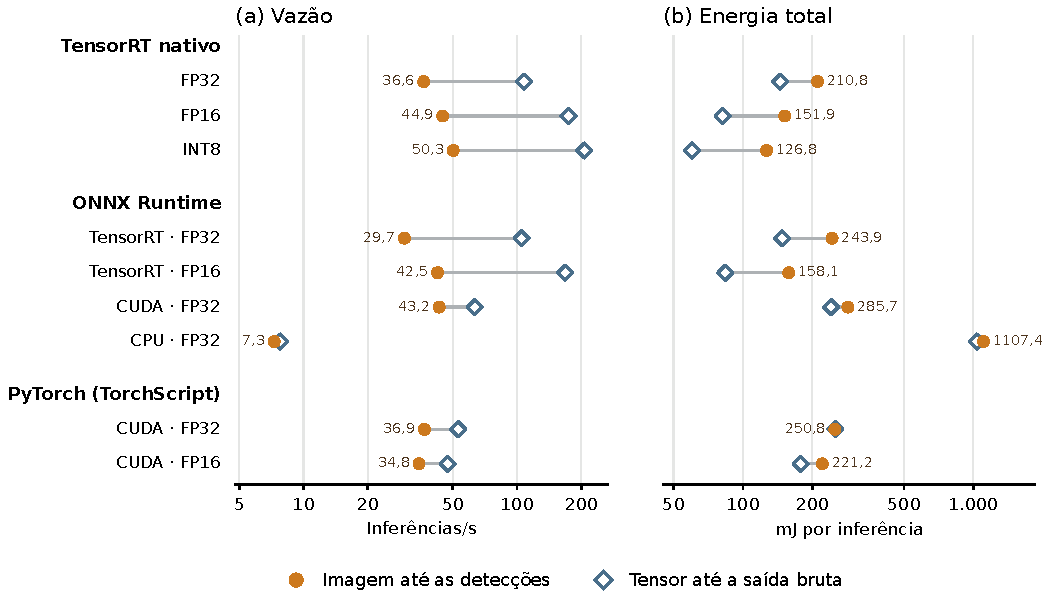
\includegraphics[width=\textwidth]{figuras/fig_bancada_vazao_energia.pdf}
  \fonte{Elaborado pelo autor a partir dos ensaios da Seção~\ref{sec_metodo_jetson}, com lote unitário e pesos COCO. Os círculos e seus rótulos mostram o processamento desde a imagem em memória até as detecções. Os losangos mostram a execução desde o tensor preparado até a saída bruta. Os dois eixos horizontais são logarítmicos. A energia total inclui a alimentação da placa em repouso.}
\end{figure}

O preparo da entrada e a conversão da saída em detecções limitam a vazão disponível para processar os recortes. Em TensorRT nativo com FP16, a taxa de 174,5~tensores/s caiu para 44,9~resultados/s quando a medição incluiu essas etapas. Com as mesmas imagens e precisão, o provedor TensorRT do ONNX Runtime entregou 42,5~resultados/s. Diferenças dessa ordem exigem cautela, pois a frequência da placa variou automaticamente entre rodadas. No TensorRT nativo em FP32, a vazão passou de 30,0~resultados/s no ensaio preliminar para 36,6 na rodada principal.

Os tempos da Figura~\ref{fig_bancada_vazao_energia} correspondem à operação após o aquecimento. No ensaio preliminar, a primeira sessão do ONNX Runtime com provedor TensorRT levou 175~s em FP32 e 526~s em FP16 para construir o motor. Na rodada principal, reutilizar o motor em \textit{cache} reduziu o carregamento para cerca de 3~s em ambas as precisões. Esse custo inicial de tempo pode ser distribuído entre os recortes processados durante a sessão.

Entre as três precisões do TensorRT nativo, FP16 reduziu em 43\% a energia por recorte acima do repouso em relação a FP32 no ensaio com 95 imagens. Ambas atingiram 41,2\% de mAP$_{50\text{--}95}$ nas 500 imagens do COCO, à precisão de uma casa decimal (Figura~\ref{fig_bancada_precisao_coco}). INT8 reduziu a energia incremental para 32,2~mJ e elevou a vazão a 50,3~inferências/s, ao custo de 5,3 pontos percentuais de mAP em relação a FP16. Esse compromisso entre consumo e qualidade motivou o uso de FP16 na projeção dos voos (Tabela~\ref{tab_jetson_configuracoes}).

\begin{figure}[!htbp]
  \centering
  \caption{Efeito da precisão numérica sobre a detecção e a energia no TensorRT nativo}
  \label{fig_bancada_precisao_coco}
  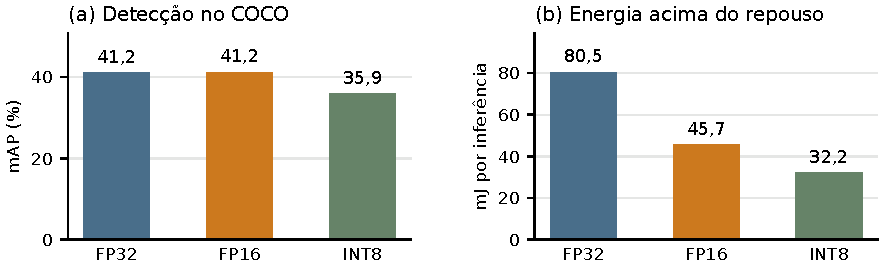
\includegraphics[width=.87\textwidth]{figuras/fig_bancada_precisao_coco.pdf}
  \fonte{Elaborado pelo autor. Em (a), a mAP$_{50\text{--}95}$ foi calculada nas mesmas 500 imagens do COCO para as três precisões. Em (b), a energia acima do repouso foi medida da imagem até as detecções nas 95 imagens da bancada. A configuração INT8 admite operações em FP16.}
\end{figure}

\begin{table}[!htbp]
  \centering
  \caption{Vazão e consumo do YOLO11n na Jetson em TensorRT FP16}
  \label{tab_jetson_configuracoes}
  \begin{tabular}{@{}lr@{}}
    \hline
    Medida & Valor \\
    \hline
    Vazão (recortes/s) & 44,87 \\
    Latência média por recorte (ms) & 22,28 \\
    Percentil 99 da latência por recorte (ms) & 23,30 \\
    Potência média da placa em repouso (W) & 4,76 \\
    Potência média da placa no ensaio (W) & 6,81 \\
    Energia por recorte acima do repouso (mJ) & 45,72 \\
    \hline
  \end{tabular}
  \fonte{Elaborado pelo autor a partir do ensaio de bancada com um recorte por inferência. A potência foi medida na entrada da placa (\texttt{VDD\_IN}).}
\end{table}

\subsection{Demanda de recortes e espera simulada na Jetson}
\label{sec_res_jetson_memoria}

Nos vídeos a 29,97 quadros/s, os quadrantes e o intervalo solicitaram em média 5,59 recortes/s, o equivalente a 12,5\% da vazão de bancada. Para acompanhar a mesma câmera, a inferência integral exigiria 719,28 recortes/s, cerca de 16 vezes a vazão medida (Figura~\ref{fig_jetson_demanda}a).

A distribuição dos recortes no tempo explica por que estratégias com a mesma demanda média entregariam resultados em prazos distintos (Figura~\ref{fig_jetson_demanda}b). Nos quadrantes, 8.191 dos 8.435 quadros selecionados enviaram um único recorte. O intervalo concentrou os envios em 368 quadros, quase sempre com 24 recortes por vez. Com processamento sequencial à latência média de bancada, a mediana do tempo entre a chegada do quadro e a conclusão de seu último recorte foi de 22~ms nos quadrantes e de 535~ms no intervalo.

Nos quadrantes, 14 envios encontraram o detector ocupado e a maior espera até o início do processamento foi de 357~ms. No intervalo, todos os envios encontraram o detector livre. As duas estratégias concluíram o processamento antes do fim de cada voo também em um segundo cenário, no qual se fixou em 23,30~ms a duração de todos os recortes. Esse valor é o percentil 99 da latência individual em bancada. A simulação com duração fixa não estima o percentil 99 da espera em voo.

\begin{figure}[!htbp]
  \centering
  \caption{Demanda de recortes nos seis voos e ocupação projetada do detector na Jetson}
  \label{fig_jetson_demanda}
  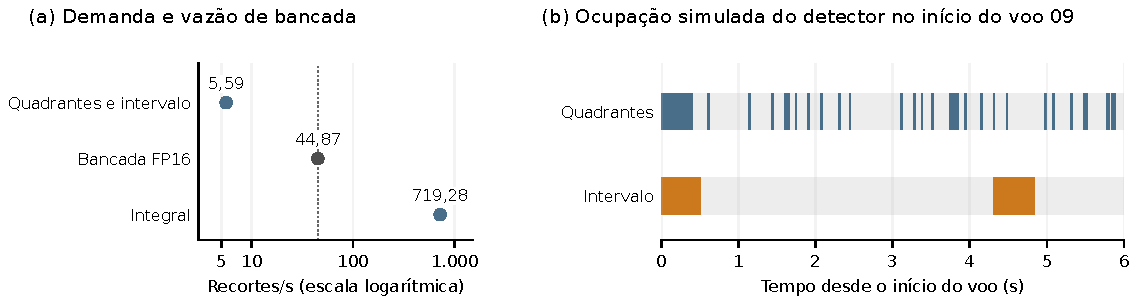
\includegraphics[width=\textwidth]{figuras/fig_jetson_quadrantes_intervalo.pdf}
  \fonte{Elaborado pelo autor a partir dos horários de envio e da Tabela~\ref{tab_jetson_configuracoes}. Em (a), a demanda é a razão entre o total de recortes e a duração dos seis voos. Em (b), as faixas coloridas mostram os períodos de processamento nos primeiros seis segundos do voo~09 e o cinza indica o tempo livre.}
\end{figure}

Como as duas estratégias concluiriam os mesmos 8.796 recortes, cada uma acrescentaria 0,112~Wh ao consumo da placa nos seis voos, admitindo que se mantenham os 45,72~mJ por recorte medidos acima do repouso. Distribuído pela duração dos voos, o acréscimo equivale a 0,26~W. Com a placa ligada durante todo o percurso, sua potência média estimada chega a 5,02~W, dos quais 4,76~W correspondem ao repouso (Equação~\eqref{eq_pc}). A projeção usa os pesos COCO e começa com a imagem em memória. Para avaliar a cadeia completa com os pesos treinados na MBG-V2, ainda é preciso medir a captura e a decodificação em 4K, a seleção dos recortes e a associação das detecções no mapa.

\section{Estimativa da energia por área com a Jetson a bordo}
\label{sec_balanco_por_voo}

Nos seis voos de teste, estimou-se quanto transportar e alimentar a Jetson acrescentaria à energia medida na bateria. A partir dessa referência, variaram-se a altura da câmera e a sobreposição entre passadas para examinar a área que cada unidade de energia permitiria imagear.

\subsection{Massa do kit e potência em cruzeiro}
\label{sec_massa_jetson}

A massa de referência do kit Jetson Orin Nano é de 174~g \cite{nvidia2023orinmass}. Os cenários de 100 e 250~g representam uma montagem mais leve e outra mais pesada, com acessórios. Em pairado, a Equação~\eqref{eq_dm} prevê aproximadamente 1,5\% a mais de potência induzida ideal para cada 1\% de massa adicional. Em cruzeiro, a carga altera a tração e a inclinação exigidas. Para calcular seu custo no numerador da Equação~\eqref{eq_coprojeto}, estimaram-se as potências com e sem a massa $m_H$, mantidos a velocidade, o arrasto da fuselagem, a rotação e o fator $\eta=0{,}836$,
\begin{equation*}
  \Delta P_{\mathrm{prop}}(V,m_H)=
  \frac{P(V;m_0+m_H)-P(V;m_0)}{\eta}.
\end{equation*}
A estimativa supõe que toda a potência fornecida pela bateria à placa chegue à sua entrada. Se houver perdas no conversor, a bateria terá de fornecer mais potência.

\begin{figure}[!htbp]
  \centering
  \caption{Potência de propulsão estimada em função da velocidade e da massa do kit}
  \label{fig_potencia_com_kit}
  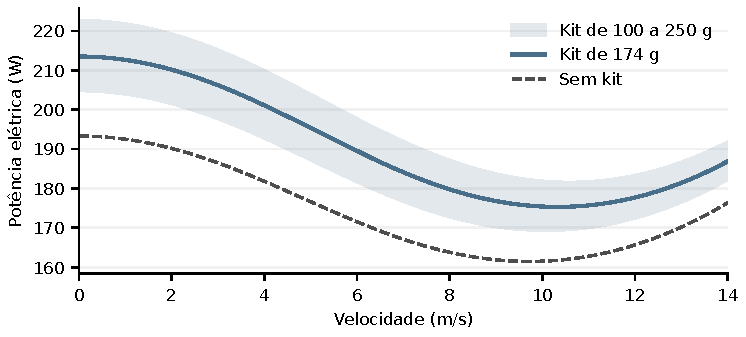
\includegraphics[width=.76\textwidth]{figuras/fig_massa_kit.pdf}
  \fonte{Elaborado pelo autor com o modelo de voo nivelado. As curvas representam a aeronave sem o kit e com o kit de 174~g. A faixa abrange as montagens de 100 a 250~g.}
\end{figure}

A 4,1~m/s e com rotação fixa, a potência de propulsão estimada sobe de 181,3~W sem o kit para 200,5~W com 174~g (Figura~\ref{fig_potencia_com_kit}). As medições da bateria foram feitas com a aeronave sem o kit. Verificar o acréscimo de potência previsto para os 174~g exige repetir o percurso com a carga instalada.

Dividindo a energia de transporte do kit pela duração total dos seis voos, obtém-se um acréscimo médio de 19,27~W na propulsão. A placa consumiria outros 4,76~W em repouso. A parcela de inferência depende do tempo de processamento, estimado a partir dos horários de envio dos recortes e da vazão medida em bancada para cada configuração (Figura~\ref{fig_potencia_estrategias_motores}).

\begin{figure}[H]
  \centering
  \caption{Acréscimo médio de potência em relação ao drone sem o kit, por estratégia e configuração da Jetson}
  \label{fig_potencia_estrategias_motores}
  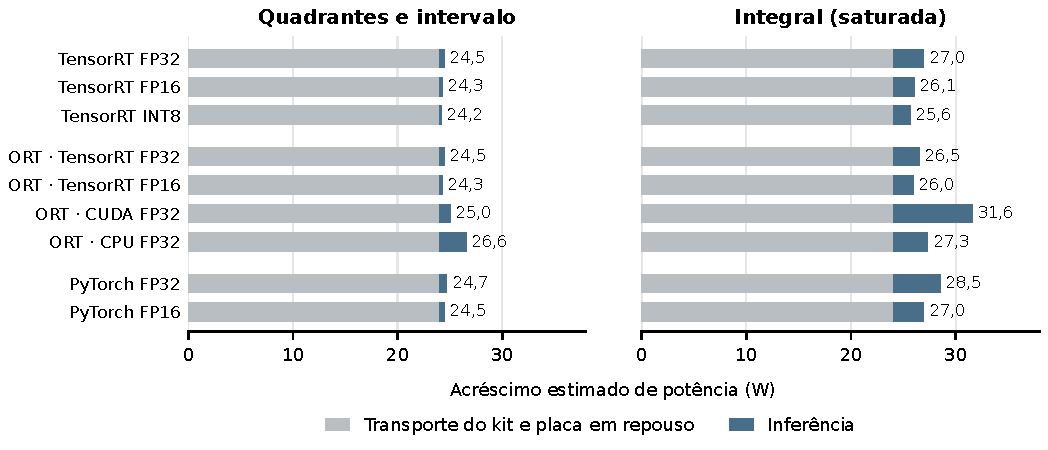
\includegraphics[width=\textwidth]{figuras/fig_potencia_estrategias_motores.pdf}
  \fonte{Elaborado pelo autor para uma Jetson com o kit de 174~g. Quadrantes e intervalo compartilham as barras porque as estimativas coincidem a uma casa decimal nas nove configurações. Na integral, a placa trabalha continuamente e a barra inclui apenas o processamento realizado durante o voo. ORT designa o ONNX Runtime. O PyTorch foi executado com TorchScript.}
\end{figure}

Em TensorRT FP16, os quadrantes e o intervalo concluiriam o processamento dos 8.796 recortes de cada estratégia. Transportar o kit e executar qualquer uma das duas estratégias consumiria 10,61~Wh adicionais nos 26,2~min de voo, o que corresponde a um acréscimo médio de 24,3~W. Na integral, a potência adicional chegaria a 26,1~W, mas a placa concluiria apenas 6,2\% dos 1.131.600 recortes até o fim dos vídeos. Mesmo a configuração mais rápida, TensorRT INT8, alcançaria 7,0\% da demanda integral.

\subsection{Consequência para a energia por área imageada}
\label{sec_exemplo_coprojeto}

Nos seis voos de teste, a bateria forneceu 80,08~Wh. A energia $E_i$ vem das medições de tensão e corrente (Equação~\eqref{eq_energia}). A área $A_i$ conta uma única vez cada célula imageada de 0,5~m de lado, com o $GSD$ ajustado por voo. As revisitas consomem energia sem ampliar essa área.

À energia medida na bateria, somaram-se a energia para transportar o kit e a energia para alimentar a placa. Para o transporte, integrou-se por trapézios a potência adicional prevista à velocidade horizontal de cada instante. Para a placa, usou-se a taxa média de recortes $r_i$. Com $E_i$ em Wh, $A_i$ em km$^2$ e $t_i$ em segundos, o custo em Wh/km$^2$ é
\begin{equation}
  e_i(m_H,r_i)=\frac{1}{A_i}\left[
      E_i + \frac{1}{3600}\int_0^{t_i}\!\Delta P_{\mathrm{prop}}\bigl(V_i(t),m_H\bigr)\,dt
      + \frac{(P_{c0}+r_iE_{\mathrm{inf}})t_i}{3600}
  \right].
  \label{eq_placa_por_area}
\end{equation}
A parcela de alimentação se anula com a placa desligada. Em repouso, $r_i=0$ e permanece $P_{c0}$. Para a placa ativa, usaram-se o TensorRT FP16 e o número de recortes enviados em cada voo, igual para os quadrantes e o intervalo.

\begin{table}[!htbp]
  \centering
  \caption{Mediana da energia por área imageada nos seis voos, sem o kit e com o kit de 174~g}
  \label{tab_balanco_telemetria}
  \begin{tabular}{@{}lr@{}}
    \hline
    Estado & Energia por área (Wh/km$^2$) \\
    \hline
    Aeronave sem o kit & 239,0 \\
    Kit transportado, placa desligada & 263,9 \\
    Placa ligada em repouso & 270,0 \\
    Placa ativa, quadrantes ou intervalo & 270,3 \\
    \hline
  \end{tabular}
  \fonte{Elaborado pelo autor. A primeira linha usa a energia medida e a área reconstruída pela telemetria. Nas demais, somaram-se os custos estimados em cada voo antes de calcular a mediana dos seis.}
\end{table}

Com o kit de 174~g ativo, a mediana da energia por área passaria de 239,0 para 270,3~Wh/km$^2$, um aumento de 13,1\% entre as duas medianas (Tabela~\ref{tab_balanco_telemetria}). Os voos 10 e 15 mostram por que um acréscimo de potência semelhante, de cerca de 24,3~W, tem custos diferentes por unidade de área (Figura~\ref{fig_energia_por_area}). O voo~10 cobriu 1,13~ha por minuto, a um custo adicional de 35,7~Wh/km$^2$. Como o voo~15 cobriu mais terreno no mesmo tempo, 1,37~ha por minuto, o acréscimo foi menor, de 29,5~Wh/km$^2$.

\begin{figure}[!htbp]
  \centering
  \caption{Energia total por área imageada em cada voo, sem o kit e com a Jetson em TensorRT FP16}
  \label{fig_energia_por_area}
  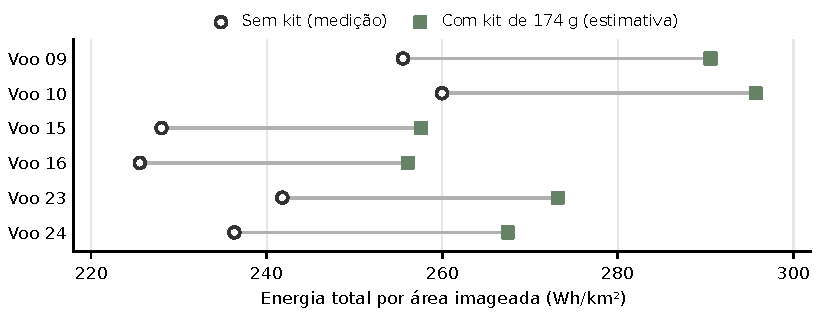
\includegraphics[width=.80\textwidth]{figuras/fig_energia_por_area.pdf}
  \fonte{Elaborado pelo autor com a telemetria da MBG-V2 e a Equação~\eqref{eq_placa_por_area}. Em cada linha, o círculo usa a energia medida na bateria e o quadrado inclui a energia estimada para transportar e alimentar o kit com o número de recortes observado nas duas estratégias. Ambos usam a mesma área imageada no voo.}
\end{figure}

Com o detector ativo em FP16, variar a massa do kit de 100 para 250~g elevaria a mediana de 259,6 para 281,6~Wh/km$^2$. Para o kit de 174~g, o transporte respondeu por 24,8~Wh/km$^2$ adicionais na mediana. A inferência em FP16 acrescentaria 0,33~Wh/km$^2$ acima do repouso, dos quais a troca para INT8 pouparia cerca de 0,10~Wh/km$^2$.

\subsubsection*{Efeito da altura simulada nos seis percursos}

\begin{figure}[!htbp]
  \centering
  \caption{Energia por área reprojetada e recall geográfico dos recipientes originais em função da altura nos seis voos}
  \label{fig_altura_percursos}
  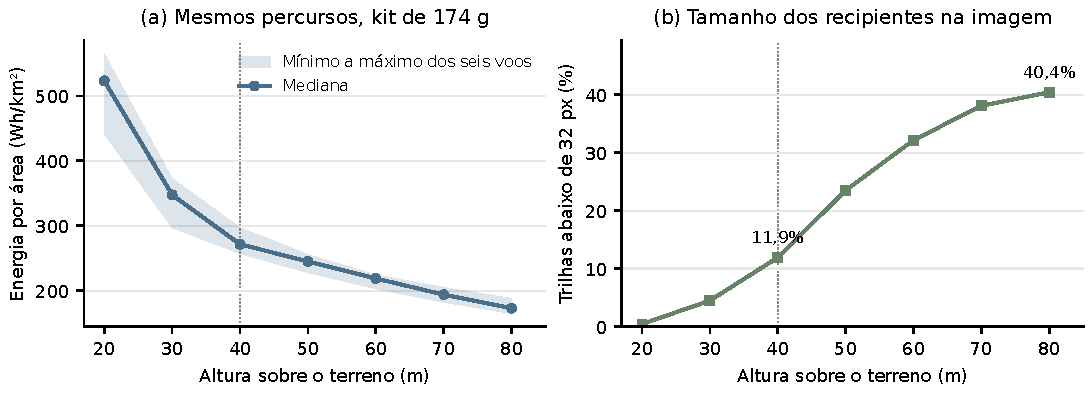
\includegraphics[width=\textwidth]{figuras/fig_altura_percursos.pdf}
  \fonte{Elaborado pelo autor com as trajetórias e anotações da MBG-V2. No painel de energia, cada percurso mantém a energia estimada para o kit ativo de 174~g. A área varia com a altura, e a faixa abrange os valores mínimo e máximo dos seis percursos. No painel de detecção, o denominador permanece em 1.924 recipientes e cada estratégia mantém os 8.796 recortes escolhidos no vídeo original. Os voos foram filmados a 40~m.}
\end{figure}

Na reprojeção dos percursos de 40 para 80~m, a mediana da energia por área caiu de 270,3 para 172,3~Wh/km$^2$ (Figura~\ref{fig_altura_percursos}). A queda de 36,3\% ficou abaixo dos 50\% previstos para uma passada retilínea isolada (Equação~\eqref{eq_e_h}), pois parte da faixa ampliada recobriu terreno já filmado. Entre os recipientes do vídeo original, os quadrantes localizaram 191 a menos na simulação a 80~m, e o intervalo, 170 a menos. Como a área reprojetada inclui terreno fora da imagem original, esses resultados não permitem calcular quantos recipientes seriam encontrados por unidade de energia em um voo real a 80~m.

\subsubsection*{Sobreposição entre passadas paralelas}

Em um levantamento com passadas paralelas longas, a separação entre as linhas determina a largura de terreno novo coberta por passada. Se $o$ é a fração de sobreposição lateral, essa largura é $d=w(h)(1-o)$. Substituindo $w$ por $d$ na Equação~\eqref{eq_e_area}, obtém-se $e=P_{el,\mathrm{tot}}/[Vw(h)(1-o)]$ em J/m$^2$. Considerou-se cruzeiro nivelado a 4,1~m/s, com 205,6~W de potência total estimada para o kit ativo. A largura de referência aos 40~m foi de 56,1~m, mediana dos seis voos. Esse cenário de planejamento representa o interior da área de levantamento, onde predominam as linhas retas e o efeito das curvas de retorno e das bordas é desprezado.

\begin{figure}[!htbp]
  \centering
  \caption{Energia por área projetada ao variar a altura e a sobreposição lateral entre passadas}
  \label{fig_altura_sobreposicao}
  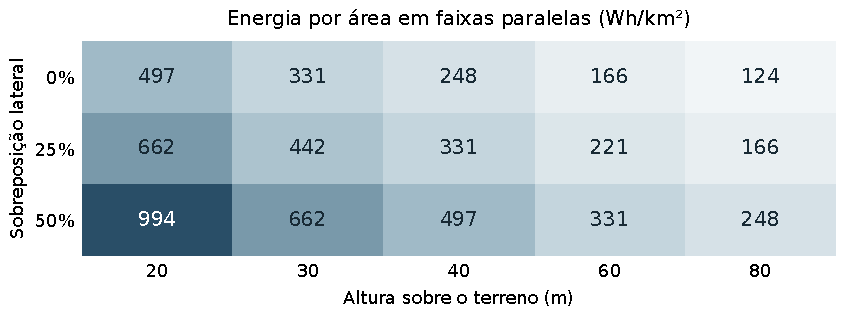
\includegraphics[width=.82\textwidth]{figuras/fig_altura_sobreposicao.pdf}
  \fonte{Elaborado pelo autor com as Equações~\eqref{eq_pegada} e~\eqref{eq_coprojeto}. Cada célula representa um plano de voo com o lado longo da imagem perpendicular ao deslocamento, o kit de 174~g ativo e a taxa média observada de 5,59~recortes/s.}
\end{figure}

A 40~m, elevar a sobreposição lateral de zero para 25\% faz o custo passar de 248 para 331~Wh/km$^2$ (Figura~\ref{fig_altura_sobreposicao}). Planos de mesmo custo também podem produzir imagens diferentes. Na altura de 80~m com 50\% de sobreposição, as linhas ficam separadas pelos mesmos 56,1~m que a 40~m sem sobreposição, e ambos os planos custam 248~Wh/km$^2$ no modelo. No voo mais alto, porém, as faixas vizinhas compartilham metade da largura e o lado de um mesmo recipiente ocupa metade dos pixels.
